
\chapter{Introduksjon}




\section{Motivasjon}
\label{sec:motivasjon}

Tale og språk tillater oss å rekke ut til andre og leve tilfredstillende liv som uavhengige medlemmer av samfunnet. Språk gir oss identitet, felleskap  og tilhørighet. Det er derimot flere som blir hindret i å uttrykke seg gjennom tradisjonelle kommunikasjonsformer på grunn av ulike funksjonshemninger  \cite{tobii}. De har derfor et behov for alternativer for å kunne kommunisere. Folk med syn eller hørselsskader har tatt i bruk gester, tegnstøtte eller tegnspåk. Andre har måttet bruke mer håndgripelige hjelpemidler. Ett kjennetegn ved disse formene for kommunikasjon er at de krever at brukeren har muskelkraft. Et krav som utelukker  personer med ALS, cerebral parese (CP), autisme og afasi eller de som har hatt hjerneslag. Folk med disse funksjonshemningene har ofte motoriske utfordringer som hindrer dem fra nettopp verbal og kroppspråklig kommunikasjon. Ved hjelp av data- og øyestyrings-teknologi er det mulig for flere av disse menneskene å kommunisere. Utfordringen er at feltet er relativt ungt og nåværende forskning har hovedsaklig blitt gjort på voksne uten funksjonshemninger (OBS! pass på at du ikke gjør det samme eller evt fjerner denne) \cite{aac}. I dette prosjektet vil fokus bli rettet mot barn som ikke har tilgang på tradisjonelle kommunikasjonsformer.




\section{Målgruppe}

I kapittel \ref{sec:motivasjon} nevnes det at det er flere unge mennesker som helt eller delvis mangler tale. Som en konsekvens av dette har de behov for andre uttrykksformer for å kommunisere. Alternative uttrykksformer kan være håndtegn, symboler eller fotografier. Slike utradisjonelle uttrykksformer går under fellesbetegnelsen alternativ og supplerende kommunikasjon (\gls{aske}).
Personer bruker ASK enten fordi det er et behov for å erstatte talen eller for å supplere utydelig eller svak tale.

International Society for Augmentative and Alternative Communication (\gls{isaac}) \cite{HvaErASK} definerer ASK som alt som hjelper en person til å kommunisere effektivt når tradisjonelle måter å kommunisere på ikke strekker til.

Målgruppen i denne avhandlingen er personer som har behov for ASK systemer. Mer spesifikk vil rapporten være rettet mot: (A) Mennesker som ikke har mulighet for tale- og kroppspråk,  (B) personer ikke håndterer skriftspråk og (C) at de er nybegynnere på symbolbasert kommunikasjon. Dette gjelder hovedsaklig barn i alderen 2 til 5 år, men også eldre med mentale begrensninger. Videre i dette prosjektet vil personer som møter disse kriteriene bli omtalt som barn med komplekse kommunikasjonsbehov. 



\section{Mål}
\label{sec:goal}

Målet med dette prosjektet er å lage et ASK-system som hjelper barn med komplekse kommunikasjonsbehov å kommunisere. Systemet som skal utvikles tar utgangspunkt i et eksisterende program som heter Sono Flex (se figur ~\ref{fig:SonoFlex}). Programmets hovedfunksjon er å konvertere tekst og symboler til tale, samt at det innholder et rikholdig utvalg av funksjoner for læring, omgivelsekontroll og elektronisk fjernkommunikasjon \cite{TobiiCommunicator}. Formålet med systemet er å hjelpe brukeren å kommunisere med symboler. Der et symbol representerer et ord eller et konsept som "hjem" eller "min mor". Problemstillingen er at når brukerens aktive vokabular vokser, så vil også antallet symboler øke. Dette gjør at det oppstår et behov for å dele symbolene inn i kategorier og flere visninger.

Light og Drager \cite{aac} argumenterer at videre forskning innen ASK teknologi må fokusere på forbedret design, for bedre å kunne møte behovet fra unge barn og eldre nybegynnere. I dette prosjektet er målet å designe og prototype mulige løsninger som reduserer den mentale belastningen på brukeren, mens han bruker et stort vokabular, med eller uten en øyestyrings enhet.

\begin{figure}[ht!]
\centering
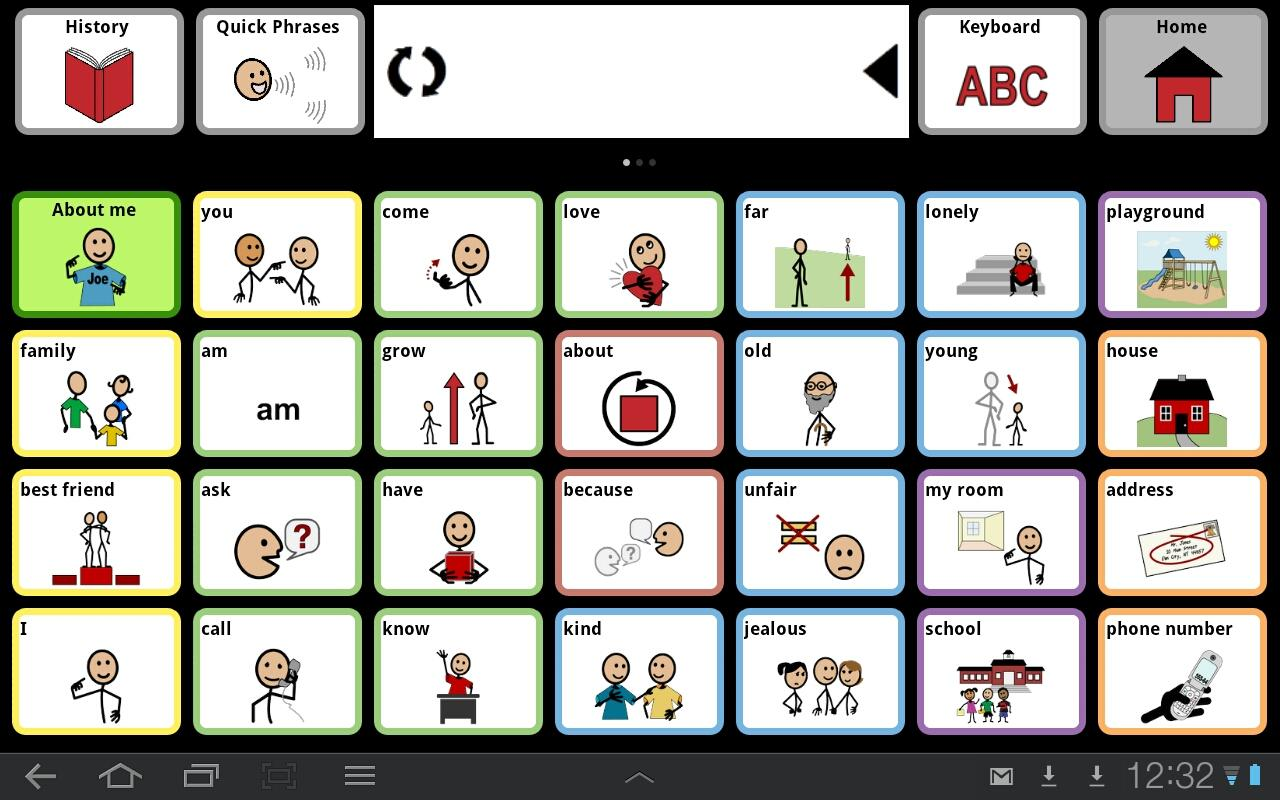
\includegraphics[width=150mm]{SonoFlex2}
\caption{Skjermdump av ASK programvaren Sono Flex}
\label{fig:SonoFlex}
\end{figure}


\section{Forskningspørsmål}
\label{sec:ResearchQuestion}

For å forske på mulige løsninger som forbedrer ASK-systemer vil en rekke funksjoner integreres i prototypen. Funksjoner som vil bli utprøvd og forsket på er følgende:


\begin{enumerate} 
\label{lst:features}
\item Forbedret visualisering. Undersøk mulige fordeler forskjellige visualisering effekter kan ha på navigering innen og mellom sider og kategorier.
\item Lydeffekter. Undersøk mulige fordeler forskjellige lydeffekter kan ha på navigering innen og mellom sider og kategorier.
\item Optimal organisering og kategorisering. Hvordan skal knapper bli organisert og kategorisert for best å legge til rette for og forenkle navigasjon
\item Brukertilpasning. Mennesker har forskjellige preferanser. Undersøk mulighetene for tilpasning av symbolstørrelse, animasjonsfart, farger o.s.v. 
\end{enumerate} 


Forskningen vil bli gjort ved å implementere et program basert på en eksisterende løsning. De ulike forbedringene beskrevet i (1),(2) og (3) vil bli integrert. Samtidig vil det også være mulighet tilpasse etter ønske (4). 


\section{Forskningsmetode}

Som nevnt i seksjon \ref{sec:ResearchQuestion}, er oppgaven å forbedre en type kommunikasjons programvare for mennesker med komplekse kommunikasjonsvansker. For å undersøke innvirkningene til de forskjellige funksjonene, vil de prøves ut på en testgruppe.
For å få til dette, vil et utvalg av deltakerene prøve systemet uten tilleggsfunksjonene, mens de gjenværende vil forsøke med funksjonene. Mens deltagerne kjører programmet vil deres interaksjon med bli automatisk lagret i logg. Informasjonen fra undersøkelsen vil vise hvordan brukeren navigerte og hvor lang tid de brukte. Dette kan igjen brukes til å verifisere om en funksjon er en forbedring eller ikke.

